\begin{frame}
    \frametitle{WP1: POC}
    \begin{block}{Case}
        \begin{itemize}
            \item Dataset: Mouse 1 - slice 153
            \item Cell type source: \textit{Astro}
            \item Cell type target: \textit{L2/3 IT}
            \item View of Anndata object: 1715 cells x 18450 genes
            \item Sample L LR interactions from \textit{mouse consensus}:\break
                5: \{(Tac2 - Tacr3), (Angpt2 - Tek), (Actr2 - Adrb2), (Tnf - Tnfrsf1a), (Angpt1 - Tek)\}
            

        \end{itemize}
    \end{block}
\end{frame}

\begin{frame}
    \frametitle{Data structure}
    Sparse COO tensors: these tensors are the Coordinate format, which is one of the
    storage formats for implementing sparse tensors. 

    In COO format, the specified element indices are stored as tuples of element
    indices and the corresponding values. In particular,
    \begin{itemize}
        \item \textbf{indices}: collected in tensor of size (ndim, nse) with type torch.int64
        \item \textbf{values}: collected in tensor of size (nse,) with int or float type
    \end{itemize}
    
    where ndim is the dimensionality of the tensor and nse is the number of specified elements.
\end{frame}

\begin{frame}
    \frametitle{Theoretical memory usage for only intralayer interactions}
    \begin{block}{Memory usage}
        The fully connected tensor is of dimension N x N x L. If we do not consider sparsity, the memory usage would be:
        \begin{equation*}
            \text{Memory usage} = N^2 \cdot L \cdot \text{size of float} = 1715^2 \cdot 5 \cdot 32 \approx 0.055 \text{ GB}
        \end{equation*}
        If we need to consider sparsity. Definitely we need it if we want to display networks.
        Sparsity can be defined by thresholding the interaction scores.
        \begin{itemize}
            \item If we consider the Xth percentile of the interaction scores for each LR pair, we
                would get the same number of non-zero elements for each LR pair.
            \item If we consider the Xth percentile of the interaction scores for all LR pairs,
                we would need to normalize the scores to make them comparable.
            \item If we consider less nodes as an aggeregate in space for each cellular type, we would consider less edges
                and therefore have less memory usage.
        \end{itemize}

    \end{block}
    Let's consider the first sparsity definition, where we threshold the interaction scores for
    each LR pair independently.

\end{frame}

\begin{frame}
    Number of non-zero elements in the whole tensor: 147'064 $\approx 0.56 \textit{GB}$
    \begin{figure}
        \centering
        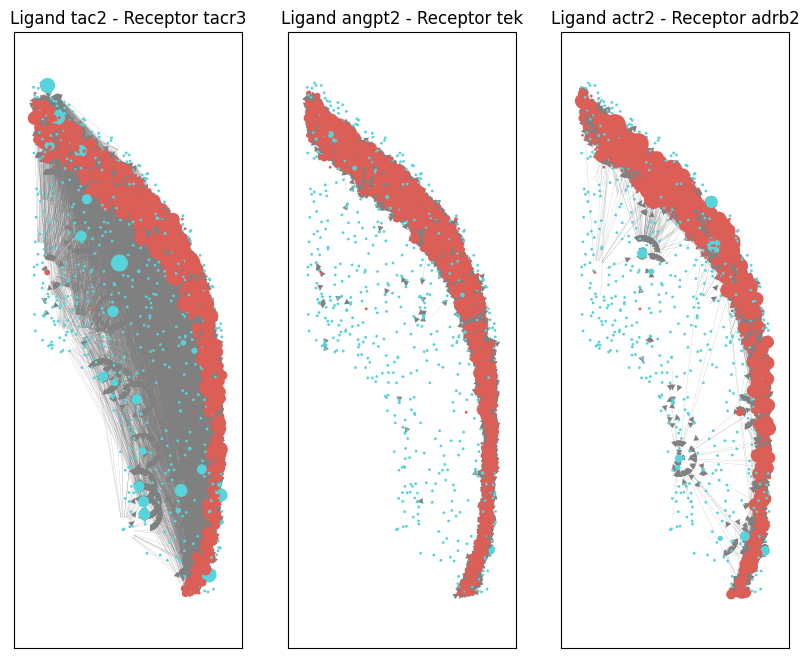
\includegraphics[width=0.7\textwidth]{media/poc_slice153_astro_l23it.png}
        \caption{Example of the 99th percentile of pairwise interaction scores for 3 different LR pairs.}
    \end{figure}

\end{frame}

\begin{frame}
    While if we consider the second sparsity definition, we would need before to zscore each LR pair.
\end{frame}


\begin{frame}
    \frametitle{How should i model the intracellular communication?}
    Let's say that the intracellular communication is modeled naively as the correlation between the receptor of 
    one layer and the ligand of another layer.

    \begin{block}{Definition}
        Let a receptor R be part of some layers of my model. For each R i will have a set
        of ligands \mathcal{L} that are ligands of other layers.

        Let's start considering the case where we evaluate the correlations between all R of one layers and L of all other layers

        More than the correlations, let's think of the product of the expression...Since we do have only a value for each cell.
    \end{block}

\end{frame}

